\documentclass{beamer}
\usetheme{metropolis}           % Use metropolis theme
\title{Exploring the role of rewiring on the structure of ecological interaction networks:\newline a simulation-based approach}
\date{July 5, 2024}
\author{Rémi Legrand}
\institute{CLBBE}

\begin{document}

\maketitle

\begin{frame}{On the importance of predicting interactions in a changing env}

  \begin{columns}
    \begin{column}{.3\linewidth}
      \includegraphics<1->[width=\linewidth]{figures_slides/biodiv_loss_giec.png}
    \end{column}
    \begin{column}{.7\linewidth}
      \includegraphics<2>[width=\linewidth]{figures_slides/temperature_raising.pdf}
    \end{column}
  \end{columns}
  \vfill
  {\scriptsize \uncover<1->{IPBES report 2019} \hfill \uncover<2->{IPCC report v5 2023}}
\end{frame}

\begin{frame}{Factors to predict interactions}

  \begin{columns}
    \begin{column}{.5\linewidth}
      %\only<3>{Salut}
      %\uncover<3>{Salut}
      \begin{itemize}
      \item<1-> \textbf{Abundances}
      \item<2-> \textbf{Trait matching} %% The influence of biogeographical and evolutionary
        %% histories on morphological trait-matching and resource specialization
        %% in mutualistic hummingbird--plant networks
      \item<3-> \textbf{Phenology}
      \item<4-> \textbf{Others}  adaptation capability (rewiring)
      \end{itemize}
    \end{column}
    \begin{column}{.5\linewidth}
      \includegraphics<1>[width=\linewidth]{figures_slides/abundance.png}%
      \includegraphics<2>[width=\linewidth]{figures_slides/trait_matching.png}%
      \includegraphics<3>[width=\linewidth]{figures_slides/phenology.png}%
      \includegraphics<4>[width=\linewidth]{figures_slides/other_rewiring.png}%
    \end{column}
  \end{columns}
\end{frame}

\section{Exploring the role of rewiring on the structure of ecological interaction networks:\newline a simulation-based approach}


\begin{frame}{Current method to compute rewiring}
\protect\hypertarget{current-method-to-compute-rewiring}{}
\begin{columns}
  \begin{column}{.5\linewidth}
    \uncover<1->{$$\beta_{dissimilarity} = \frac{|a|+|c|+|b|}{\frac{|a|}{2} + |c|+ \frac{|b|}{2}} - 1$$}
    \uncover<2->{$$\beta_{WN} = \beta_{ST} + \beta_{OS}$$}\vspace{-1em}
    \uncover<3->{$$\Delta\beta_{OS,i} = \beta_{OS} - \beta_{OS,\Delta i}$$}
  \end{column}
  \begin{column}{.5\linewidth}
    \includegraphics<1->[width=\linewidth]{figures_slides/beta_div.png}%
  \end{column}
\end{columns}
\end{frame}

\begin{frame}{How do we plan to study rewiring : AFC}
\protect\hypertarget{How-do-we-plan-to-study-rewiring-:-AFC}{}
\begin{columns}
  \begin{column}{.5\linewidth}
    \includegraphics<1->[width=\linewidth]{figures_slides/network.png}%
  \end{column}
  \begin{column}{.5\linewidth}
    \includegraphics<2->[width=\linewidth]{figures_slides/AFC}%
  \end{column}
\end{columns}
\end{frame}
\begin{frame}{Foucart CA}
\protect\hypertarget{foucart-ca}{}
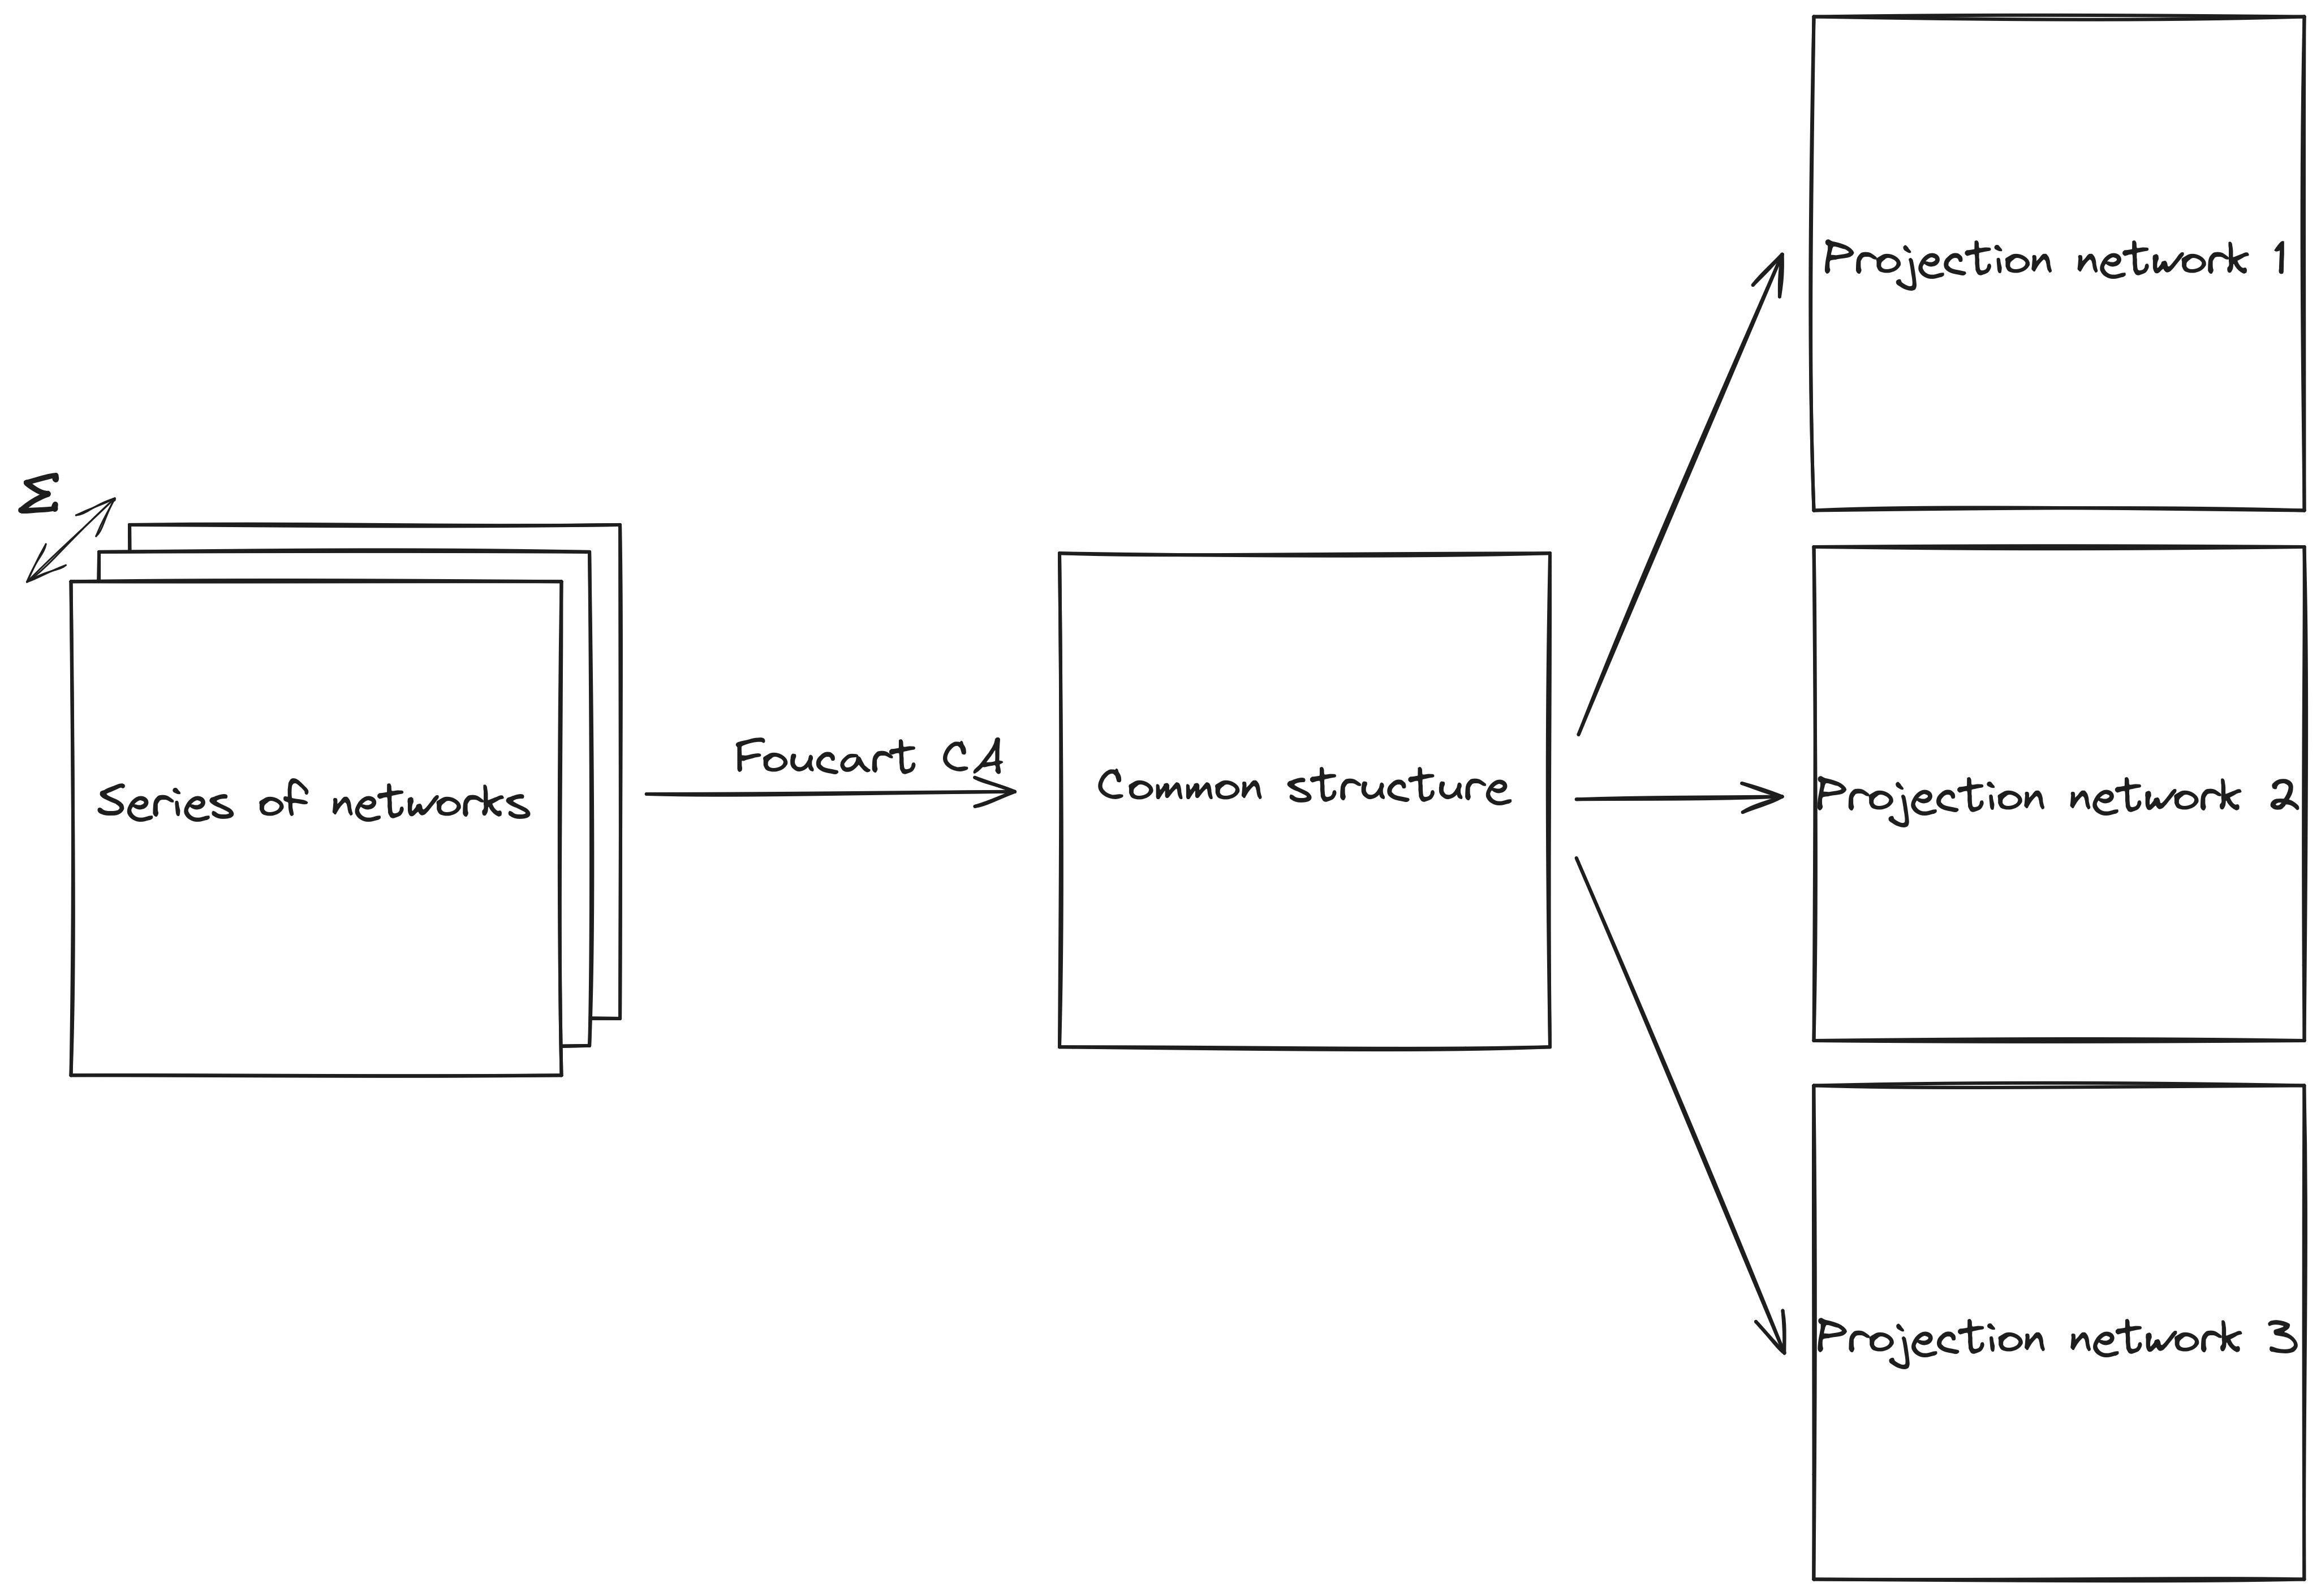
\includegraphics[width=\linewidth]{figures_slides/foucart.png}%
\end{frame}

\begin{frame}{Compare to other methods and why it did not work}
  \framesubtitle{(or did it?)}
  compare to toju and to tolerance
\end{frame}

\begin{frame}{Why it did not work}
\begin{itemize}
\item
  schematics: disappearance of species -\textgreater{} new interactions
  less favourable (not taken into account in simulated data)
\item
  schematics: reconstruction of the trait and not profile interaction
  (the id of the interactant does not matter)
\end{itemize}
\end{frame}

\begin{frame}{Perspectives to improve beta diversity and further
research on Foucart}
\protect\hypertarget{perspectives-to-improve-beta-diversity-and-further-research-on-foucart}{}
\begin{itemize}
\item
  how to compute better the beta dissimilarity: take into account the
  abundances and not just the presence/ abscence of the species in the
  different networks
\item
  a simulation bias? : resilience to perturbation not taken into account
  in the simulation
\end{itemize}
\end{frame}

\begin{frame}{Citations:}
\protect\hypertarget{citations}{}
\begin{itemize}
\item
  Image giec biodiv: Figure 2.6 in Parmesan, C., M.D. Morecroft, Y.
  Trisurat, R. Adrian, G.Z. Anshari, A. Arneth, Q. Gao, P. Gonzalez, R.
  Harris, J. Price, N. Stevens, and G.H. Talukdar, 2022: Terrestrial and
  Freshwater Ecosystems and their Services. In: Climate Change 2022:
  Impacts, Adaptation, and Vulnerability. Contribution of Working Group
  II to the Sixth Assessment Report of the Intergovernmental Panel on
  Climate Change {[}H.-O. Pörtner, D.C. Roberts, M. Tignor, E.S.
  Poloczanska, K. Mintenbeck, A. Alegría, M. Craig, S. Langsdorf, S.
  Löschke, V. Möller, A. Okem, B. Rama (eds.){]}. Cambridge University
  Press, Cambridge, UK and New York, NY, USA, pp. 197-377,
  doi:10.1017/9781009325844.004.
  \href{https://www.ipcc.ch/report/ar6/wg2/figures/chapter-2/figure-2-006}{https://www.ipcc.ch/report/ar6/wg2/figures/chapter-2/figure-2-006}
\item
\end{itemize}
\end{frame}
\end{document}
